\chapter{Regulação da pressão arterial e exercício}\label{ch:b2:blood-pressure}

Levante-se depressa depois de estar deitado e, por um segundo, meio
litro de \omterm{def:b2:blood-circulation:blood}{sangue} escoa para as \omterm{def:b2:blood-circulation:vessels}{veias} das pernas; o \omterm{def:b2:heart:anatomy}{coração}, recebendo
menos, bombeia menos, a pressão na cabeça cai, e o encéfalo --- que fica
\qty{40}{cm} acima do \omterm{def:b2:heart:anatomy}{coração} e não consegue armazenar oxigênio --- está a um
ou dois segundos de desmaiar. Isso quase nunca acontece, porque, em um
único batimento, um reflexo contraiu as \omterm{def:b2:blood-circulation:vessels}{arteríolas} e acelerou o
\omterm{def:b2:heart:anatomy}{coração}. Corra atrás de um ônibus, e os músculos precisam de dez vezes
o \omterm{def:b2:blood-circulation:blood}{sangue} que tinham em repouso; eles o recebem em um minuto, e a pressão
que o impulsiona se mantém estável enquanto a resistência do corpo
inteiro cai dois terços. Este capítulo trata dessa regulação: o que
fixa a pressão, como ela é percebida, o reflexo rápido e os hormônios
lentos que a corrigem, e como o sistema é reorganizado, e não
sobrepujado, pelo exercício.

\section{O que é a pressão}

\begin{theorem}[A equação da circulação]\label{thm:b2:blood-pressure:equation}
\index{pressão arterial média}\index{resistência periférica total}
A \omterm{thm:b2:blood-pressure:equation}{pressão arterial média} $\bar P$ é o produto do que o \omterm{def:b2:heart:anatomy}{coração} introduz
pelo que os vasos deixam sair:
\[
\bar P - P_{\text{ven}} = Q\,R, \qquad Q = f\times V_s,
\]
em que $Q$ é o \omterm{thm:b2:heart:starling}{débito cardíaco} (frequência cardíaca $f$ vezes \omterm{prop:b2:heart:cycle}{volume
sistólico} $V_s$), $R$ a \omterm{thm:b2:blood-pressure:equation}{resistência periférica total} --- as \omterm{def:b2:blood-circulation:vessels}{arteríolas}
de todos os órgãos em paralelo --- e $P_{\text{ven}}$ a pressão venosa,
próxima de zero. Em repouso, $\qty{5}{L/min}\times\qty{1.08}{mmHg.s/mL}$
dá \qty{90}{mmHg}. Toda regulação da pressão age sobre uma de três
grandezas: a frequência, o \omterm{prop:b2:heart:cycle}{volume sistólico} (por meio do enchimento e
da contratilidade do \cref{ch:b2:heart}) ou a resistência (por meio do raio
arteriolar, na quarta potência). Como os órgãos estão em paralelo, o
fluxo para cada um é sua parcela da pressão dividida por sua própria
resistência: dilatar as \omterm{def:b2:blood-circulation:vessels}{arteríolas} de um órgão aumenta seu fluxo sem
mudar o dos outros, desde que a pressão seja mantida --- e manter a
pressão é a razão de ser da regulação.
\end{theorem}
\begin{proof}
A lei de Ohm para um fluido: o fluxo através de uma resistência é a
queda de pressão através dela dividida pela resistência (Poiseuille,
\cref{ch:b2:blood-circulation}); para resistências em paralelo, os fluxos se somam e
$1/R = \sum 1/R_i$. A pressão média ao longo de um batimento é
aproximadamente a diastólica mais um terço da \omterm{thm:b2:blood-circulation:windkessel}{pressão de pulso}:
$80 + 40/3 = \qty{93}{mmHg}$.
\end{proof}

\begin{omfigure}
\begin{tikzpicture}[every node/.style={font=\scriptsize}, >=stealth]
  \node[draw, rounded corners, fill=omThm!15, minimum width=2.4cm, minimum height=1cm, align=center] (heart) at (0,0) {coração\\$Q = f\,V_s$};
  \draw[very thick, omThm] (1.2,0) -- (2.4,0);
  \draw[very thick, omThm] (2.4,-2.4) -- (2.4,2.4);
  \foreach \y/\org/\r in {2.0/{encéfalo}/{$R_1$}, 1.0/{músculo cardíaco}/{$R_2$}, 0/{intestino e fígado}/{$R_3$}, -1.0/{rins}/{$R_4$}, -2.0/{músculos, pele}/{$R_5$}} {
    \draw[very thick, omThm] (2.4,\y) -- (3.6,\y);
    \draw[thick, decorate, decoration={zigzag, segment length=4pt, amplitude=2pt}] (3.6,\y) -- (5.0,\y);
    \node[above] at (4.3,\y+0.05) {\org};
    \node[below] at (4.3,\y-0.05) {\r};
    \draw[very thick, omDef] (5.0,\y) -- (6.2,\y);
  }
  \draw[very thick, omDef] (6.2,-2.4) -- (6.2,2.4);
  \draw[very thick, omDef] (6.2,0) -- (7.4,0) |- (0,-3.2) -- (0,-0.5);
  \node[omThm, above] at (1.8,0.05) {$\bar P$};
  \node[omDef, below] at (3.7,-3.2) {veias, $P_{\text{ven}} \approx 0$};
  \node[anchor=west, align=left] at (7.8,1.5) {órgãos em paralelo:\\$1/R = \sum 1/R_i$\\fluxo para o órgão $i$: $\bar P/R_i$};
\end{tikzpicture}

{\small A circulação como um circuito: uma bomba, uma pressão e as
resistências arteriolares dos órgãos em paralelo. Cada órgão recebe
$\bar P/R_i$; a regulação mantém $\bar P$ enquanto as $R_i$ são
ajustadas à demanda.}
\end{omfigure}

\begin{proposition}[Por que a pressão precisa ser regulada]\label{prop:b2:blood-pressure:why}
Baixa demais, e o encéfalo --- \qty{40}{cm} acima do \omterm{def:b2:heart:anatomy}{coração} num adulto de
pé, o que custa \qty{31}{mmHg} de coluna hidrostática --- e o próprio
músculo cardíaco ficam mal irrigados: o encéfalo falha em segundos. Alta
demais, e os vasos são danificados: a parede arterial se espessa e
enrijece, os glomérulos do rim cicatrizam, a retina sangra e o \omterm{def:b2:heart:anatomy}{coração}
trabalha contra a pressão até entrar em insuficiência. A pressão também
precisa permanecer estável enquanto as demandas dos órgãos mudam em uma
ordem de grandeza --- o intestino após uma refeição, os músculos no
exercício, a pele no calor --- e enquanto o próprio volume sanguíneo se
perde numa hemorragia ou no suor. Dois sistemas fazem isso: um reflexo
nervoso que age, em um batimento, sobre a frequência, o \omterm{prop:b2:heart:cycle}{volume
sistólico} e a resistência, e sistemas hormonais que agem, ao longo de
horas e dias, sobre a resistência e, sobretudo, sobre o volume
sanguíneo, por meio do rim.
\end{proposition}

\begin{omfigure}
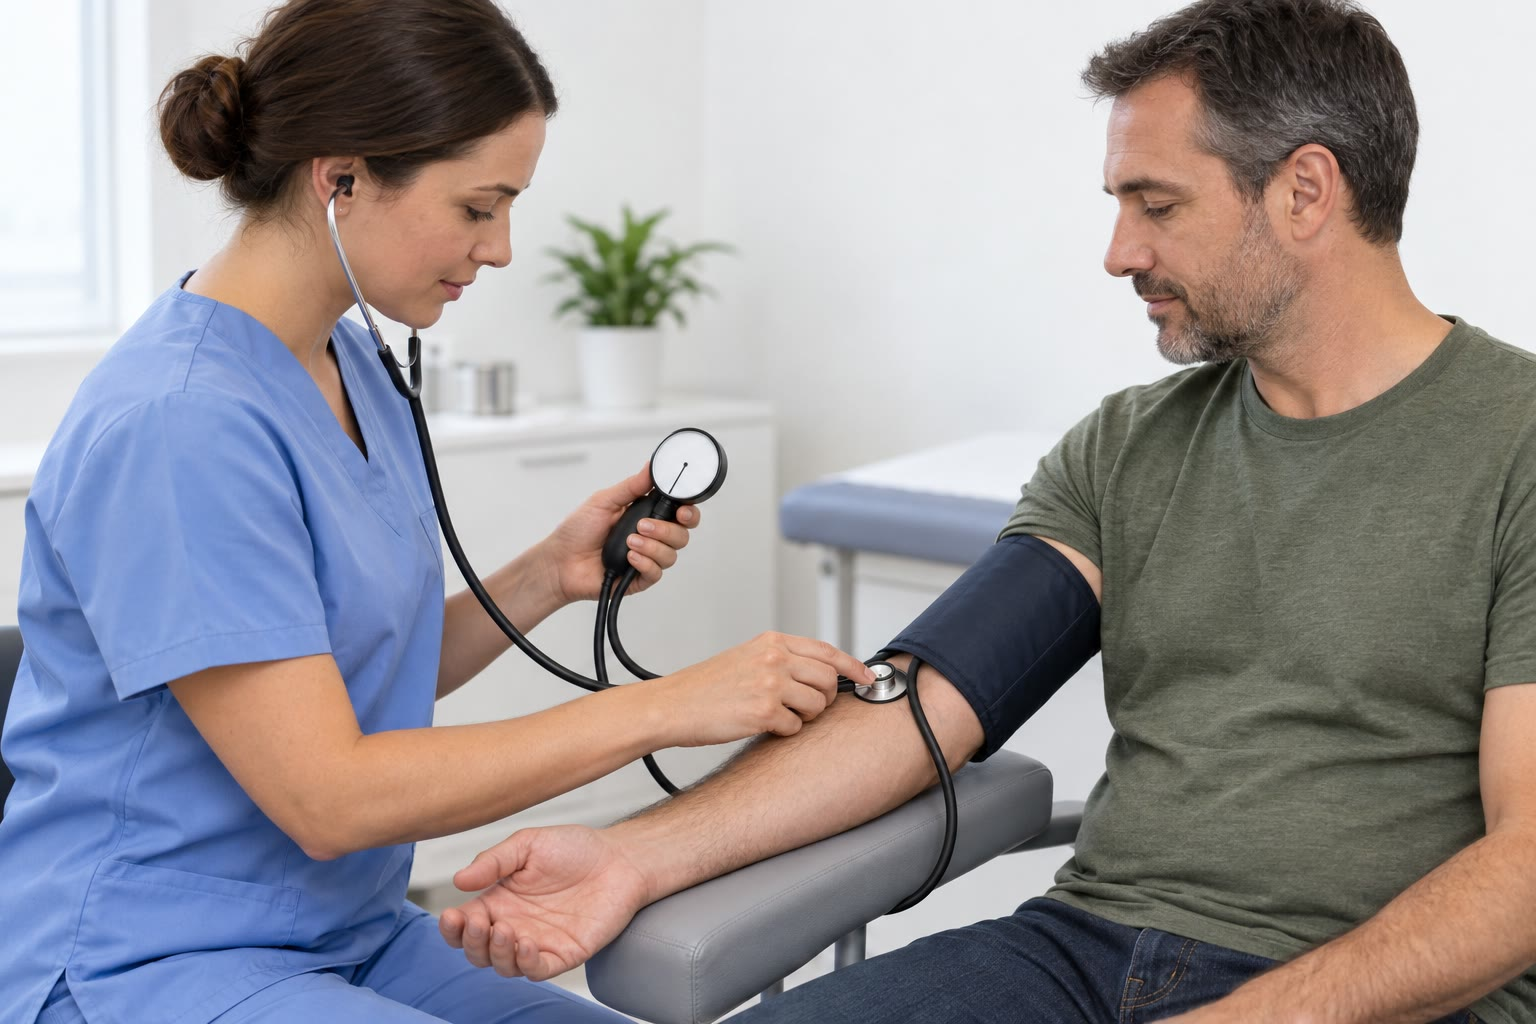
\includegraphics[width=0.6\linewidth]{images/book4/ai/b4-18-blood-pressure-cuff.jpg}

{\small A medida da pressão. O manguito é inflado acima da pressão
sistólica, de modo que nenhum \omterm{def:b2:blood-circulation:blood}{sangue} passa; à medida que é esvaziado,
os primeiros sons do escoamento turbulento sob o estetoscópio marcam a
pressão sistólica, e seu desaparecimento, quando a \omterm{def:b2:blood-circulation:vessels}{artéria} permanece
aberta durante todo o ciclo, marca a diastólica.}
\end{omfigure}

\section{A alça rápida: o barorreflexo}

\begin{definition}[O barorreflexo]\label{def:b2:blood-pressure:baroreflex}
\index{barorreceptor}\index{barorreflexo}\index{centro vasomotor}\index{sistema nervoso autônomo}
Receptores de estiramento nas paredes dos seios carotídeos (na
bifurcação de cada \omterm{def:b2:blood-circulation:vessels}{artéria} carótida, abaixo da mandíbula) e do arco
aórtico --- os \emph{barorreceptores} --- disparam a uma frequência que
aumenta com a pressão que os distende, mais depressa quando a pressão
está subindo. Seus nervos chegam aos \emph{centros cardiovasculares} do
bulbo, que controlam os dois ramos da eferência autônoma: o vago, cuja
acetilcolina desacelera o \omterm{prop:b2:heart:conduction}{nó sinoatrial}, e os nervos simpáticos, cuja
noradrenalina acelera o nó, fortalece o \omterm{def:b2:heart:anatomy}{ventrículo}, contrai as
\omterm{def:b2:blood-circulation:vessels}{arteríolas} (elevando $R$) e contrai as \omterm{def:b2:blood-circulation:vessels}{veias} (empurrando o \omterm{def:b2:blood-circulation:blood}{sangue}
armazenado em direção ao \omterm{def:b2:heart:anatomy}{coração} e aumentando o enchimento). Uma
elevação da pressão aumenta os disparos dos barorreceptores, o que
excita o vago e inibe a eferência simpática: a frequência cai, as
\omterm{def:b2:blood-circulation:vessels}{arteríolas} relaxam, a pressão baixa. Uma queda faz o inverso. A alça é
uma \emph{retroalimentação negativa} com um valor de referência perto
de \qty{95}{mmHg}, um atraso de cerca de um segundo e um ganho tal que
uma perturbação é corrigida até um quinto de seu tamanho: é a razão
pela qual você não desmaia ao se levantar.
\end{definition}
\begin{proof}[Evidências]
Hering (1923) verificou que pressionar o seio carotídeo desacelerava o
\omterm{def:b2:heart:anatomy}{coração} e baixava a pressão, e que seccionar o nervo do seio abolia a
resposta. Perfundir um seio carotídeo isolado a pressões fixas enquanto
se registrava a pressão arterial do animal deu a curva sigmoide do
reflexo: a pressão do animal cai à medida que a pressão no seio é
elevada, de modo acentuado em torno de \qty{100}{mmHg} e pouco fora de
\qtyrange{60}{160}{mmHg}. Cães com os nervos do seio e da aorta
seccionados mantêm uma pressão média normal ao longo de dias, mas
extremamente variável de um minuto para outro --- o reflexo é um
amortecedor, e não o que fixa o nível de longo prazo.
\end{proof}

\begin{omfigure}
\begin{tikzpicture}[every node/.style={font=\scriptsize}, >=stealth]
  \node[draw, rounded corners, fill=omDef!15, align=center] (bp) at (0,0) {pressão arterial\\$\bar P$};
  \node[draw, rounded corners, fill=omDef!15, align=center] (baro) at (4.2,0) {barorreceptores\\seio carotídeo, arco aórtico\\disparos $\uparrow$ com $\bar P$};
  \node[draw, rounded corners, fill=omProp!20, align=center] (med) at (8.6,0) {bulbo:\\centros cardiovasculares};
  \node[draw, rounded corners, fill=omThm!15, align=center] (vag) at (8.6,-2.2) {vago $\uparrow$: frequência $\downarrow$};
  \node[draw, rounded corners, fill=omThm!15, align=center] (sym) at (4.2,-2.2) {simpático $\downarrow$: frequência, contratilidade,\\tônus arteriolar e venoso $\downarrow$};
  \draw[->, thick] (bp) -- (baro); \draw[->, thick] (baro) -- (med);
  \draw[->, thick] (med) -- (vag); \draw[->, thick] (med) -- (sym);
  \draw[->, thick] (sym.west) -| (bp.south) node[pos=0.75, left, align=right] {$Q\downarrow$, $R\downarrow$:\\$\bar P\downarrow$};
  \draw[->, thick] (vag.west) -- (sym.east);
  \node[anchor=north, align=center] at (4.3,-3.2) {uma elevação da pressão é respondida por uma queda: retroalimentação negativa, atraso de um segundo};
\end{tikzpicture}

{\small O \omterm{def:b2:blood-pressure:baroreflex}{barorreflexo}. Uma elevação da pressão arterial aumenta os
disparos dos \omterm{def:b2:blood-pressure:baroreflex}{barorreceptores}, o que leva o bulbo a desacelerar o \omterm{def:b2:heart:anatomy}{coração}
e relaxar os vasos; uma queda faz o contrário.}
\end{omfigure}

\begin{theorem}[O ganho de uma alça de retroalimentação negativa]\label{thm:b2:blood-pressure:gain}
\index{ganho de retroalimentação}
Se uma perturbação mudaria a pressão, sem regulação, em $\Delta P_0$, e
a alça responde a qualquer desvio $\Delta P$ com uma correção de
$-G\,\Delta P$ (o \emph{ganho de alça aberta} $G$), o desvio que resta
depois que a alça agiu é
\[
\Delta P = \frac{\Delta P_0}{1 + G}.
\]
O \omterm{def:b2:blood-pressure:baroreflex}{barorreflexo} tem $G \approx 4$: levantar-se, o que baixaria a pressão
no \omterm{def:b2:heart:anatomy}{coração} em cerca de \qty{40}{mmHg}, a baixa em \qty{8}{mmHg}; uma
hemorragia que reduziria a pressão à metade a baixa em um décimo --- até
que a perda ultrapasse o que vasos mais contraídos e um \omterm{def:b2:heart:anatomy}{coração} mais
rápido conseguem disfarçar. O reflexo não abole uma perturbação; ele a
divide por cinco. E ele se \emph{reajusta}: mantidos numa nova pressão
durante horas, os \omterm{def:b2:blood-pressure:baroreflex}{barorreceptores} se adaptam e defendem o novo nível, e
é por isso que o reflexo não consegue curar a hipertensão e que o nível
de longo prazo é fixado em outro lugar.
\end{theorem}
\begin{proof}
O desvio final é a perturbação mais a correção:
$\Delta P = \Delta P_0 - G\,\Delta P$, donde $\Delta P(1 + G) =
\Delta P_0$. Com $G = 4$, $\Delta P = \Delta P_0/5$.
\end{proof}

\begin{omfigure}
\begin{tikzpicture}
\begin{axis}[
  width=0.7\linewidth, height=5.4cm,
  axis x line=bottom, axis y line=left,
  xmin=40, xmax=180, ymin=40, ymax=160,
  xlabel={pressão no seio carotídeo (\unit{mmHg})}, ylabel={pressão arterial resultante (\unit{mmHg})},
  xlabel style={font=\small, at={(axis description cs:0.5,-0.13)}, anchor=north},
  ylabel style={font=\small},
  tick label style={font=\small}, xtick={60,100,140}, ytick={60,100,140},
  clip=false,
]
\addplot[very thick, omDef, domain=40:180, samples=80] {100 + 50*tanh((100-x)/25)};
\addplot[thick, dashed, gray, domain=40:180, samples=2] {x};
\fill[omDef] (axis cs:100,100) circle (2pt); \draw[gray] (axis cs:101,100) -- (axis cs:124,110); \node[font=\scriptsize, anchor=west] at (axis cs:125,110) {valor de referência};
\node[font=\scriptsize, anchor=west, align=left] at (axis cs:46,112) {inclinação $-G$\\perto do valor de referência};
\end{axis}
\end{tikzpicture}

{\small A curva do \omterm{def:b2:blood-pressure:baroreflex}{barorreflexo}: a pressão em que o corpo se estabiliza
quando o seio isolado é mantido a uma dada pressão. Sua inclinação no
valor de referência é o ganho; fora de \qtyrange{60}{160}{mmHg}, o
reflexo está saturado.}
\end{omfigure}

\section{As alças lentas: os hormônios e o rim}

\begin{proposition}[Renina, angiotensina, aldosterona e o volume]\label{prop:b2:blood-pressure:raas}
\index{sistema renina--angiotensina}\index{aldosterona}\index{hormônio antidiurético}\index{peptídeo natriurético}
Ao longo de horas e dias, a pressão é fixada pelo \emph{volume
sanguíneo}, e o volume, pelo rim. Quando a pressão ou o sódio que chega
ao rim cai, ou quando os nervos simpáticos disparam, células das
\omterm{def:b2:blood-circulation:vessels}{arteríolas} do rim liberam no \omterm{def:b2:blood-circulation:blood}{sangue} a enzima \emph{renina}; a renina
corta uma proteína plasmática em \emph{angiotensina I}, que uma enzima
dos \omterm{def:b2:blood-circulation:vessels}{capilares} pulmonares converte em \emph{angiotensina II} --- o mais
potente vasoconstritor do corpo, que eleva $R$ em minutos, e um hormônio
que faz o córtex suprarrenal secretar \emph{aldosterona}, a qual faz o
rim reter sódio, e com ele água, nos dias seguintes. O \emph{\omterm{prop:b2:blood-pressure:raas}{hormônio
antidiurético}} da hipófise (vasopressina), liberado quando o \omterm{def:b2:blood-circulation:blood}{sangue} fica
concentrado ou seu volume cai, faz o rim reter água diretamente e
também contrai os vasos. E, quando os \omterm{def:b2:heart:anatomy}{átrios} são distendidos demais por
um volume excessivo, eles secretam \emph{\omterm{prop:b2:blood-pressure:raas}{peptídeo natriurético}}, que
faz o rim excretar sódio e água. O rim é, assim, o árbitro final: ele
pode excretar ou reter litros, e uma pressão que persiste acima do
valor de referência do rim é corrigida, ao longo de dias, pela perda de
volume --- a menos que o próprio valor de referência do rim esteja
elevado, e é isso que é a maior parte das hipertensões. (A maquinaria
própria do rim é o assunto do volume do Ano 3.)
\end{proposition}
\begin{proof}[Evidências]
Goldblatt (1934) estreitou a \omterm{def:b2:blood-circulation:vessels}{artéria} de um dos rins de um cão: o animal
se tornou hipertenso em poucos dias e assim permaneceu; verificou-se que
o rim mal irrigado liberava renina, e sua remoção curava o animal. Os
fármacos que bloqueiam a conversão da angiotensina (inibidores da ECA)
ou seu receptor baixam a pressão da maioria dos hipertensos, e um rim
transplantado de uma linhagem de ratos hipertensos torna hipertenso um
receptor normal.
\end{proof}

\begin{omfigure}
\begin{tikzpicture}[every node/.style={font=\scriptsize}, >=stealth]
  \node[draw, rounded corners, fill=omDef!15, align=center] (fall) at (0,0) {a pressão ou o volume cai;\\os nervos simpáticos disparam};
  \node[draw, rounded corners, fill=omProp!20, align=center] (renin) at (4.4,0) {o rim libera\\renina};
  \node[draw, rounded corners, fill=omProp!20, align=center] (ang) at (8.6,0) {angiotensina II\\(formada no sangue e no pulmão)};
  \node[draw, rounded corners, fill=omThm!15, align=center] (vc) at (8.6,-2.0) {vasoconstrição:\\$R\uparrow$ em minutos};
  \node[draw, rounded corners, fill=omThm!15, align=center] (ald) at (4.4,-2.0) {aldosterona (suprarrenal):\\Na$^+$ e água retidos\\em dias --- volume $\uparrow$};
  \draw[->, thick] (fall) -- (renin); \draw[->, thick] (renin) -- (ang);
  \draw[->, thick] (ang) -- (vc); \draw[->, thick] (ang) -- (ald);
  \draw[->, thick] (ald.west) -| (fall.south) node[pos=0.85, left, align=right] {pressão\\restabelecida};
  \draw[->, thick] (vc.west) -- (ald.east);
  \node[draw, rounded corners, fill=omExo!25, align=center] (anp) at (0,-2.0) {átrios distendidos:\\peptídeo natriurético,\\sal e água excretados};
  \draw[->, thick, dashed] (anp.north) -- (fall.south);
\end{tikzpicture}

{\small A alça lenta. Uma queda de pressão desencadeia a renina, a
angiotensina II e a aldosterona: constrição em minutos, retenção de sal
e de água em dias. O excesso de volume é respondido pelo \omterm{prop:b2:blood-pressure:raas}{peptídeo
natriurético} dos \omterm{def:b2:heart:anatomy}{átrios}.}
\end{omfigure}

\begin{example}[Uma hemorragia]\label{ex:b2:blood-pressure:haemorrhage}
Um doador dá \qty{500}{mL}, um décimo do \omterm{def:b2:blood-circulation:blood}{sangue}. Em segundos, o
\omterm{def:b2:blood-pressure:baroreflex}{barorreflexo} contrai as \omterm{def:b2:blood-circulation:vessels}{arteríolas} e as \omterm{def:b2:blood-circulation:vessels}{veias} e acelera o \omterm{def:b2:heart:anatomy}{coração}: a
pressão quase não se altera, a pele fica pálida e fria (suas \omterm{def:b2:blood-circulation:vessels}{arteríolas}
se fecharam), o pulso fica mais rápido. Em minutos, a pressão \omterm{def:b2:blood-circulation:vessels}{capilar}
reduzida deixa o líquido intersticial passar para os vasos (o
equilíbrio de Starling do \cref{ch:b2:blood-circulation}), restaurando metade do volume até a
hora seguinte; a renina, a angiotensina e o \omterm{prop:b2:blood-pressure:raas}{hormônio antidiurético}
reduzem a urina a um fio, e vem a sede; ao longo de dias, o rim retém
sal e água e o volume plasmático se recompõe, e ao longo de semanas a
medula óssea repõe as \omterm{def:b2:blood-circulation:blood}{hemácias}. Uma perda de \qty{2}{L} supera tudo
isso: o reflexo fica saturado, a pressão desaba, os tecidos mal
irrigados liberam lactato e os \omterm{def:b2:blood-circulation:vessels}{capilares} vazam --- é o choque, do qual
só uma transfusão tira o paciente.
\end{example}

\section{O exercício: o sistema reorganizado}

\begin{proposition}[O exercício]\label{prop:b2:blood-pressure:exercise}
\index{fisiologia do exercício}\index{fluxo sanguíneo muscular}\index{débito cardíaco!no exercício}
No exercício intenso, o consumo de oxigênio dos músculos esqueléticos
aumenta vinte vezes, e seu fluxo sanguíneo passa de \qty{1}{L/min} a
\qty{20}{L/min}. Três coisas acontecem ao mesmo tempo. Localmente, os
metabólitos do músculo em atividade --- $\mathrm{CO_2}$, lactato,
adenosina, potássio, calor, pouco oxigênio --- relaxam suas \omterm{def:b2:blood-circulation:vessels}{arteríolas}
(\emph{vasodilatação metabólica}) e abrem os \omterm{def:b2:blood-circulation:vessels}{capilares}, reduzindo a
resistência do músculo a um décimo. Centralmente, um comando do córtex
motor para o bulbo, reforçado por sinais dos próprios receptores
musculares, reajusta o \omterm{def:b2:blood-pressure:baroreflex}{barorreflexo} para um valor de referência mais
alto e ativa a eferência simpática: frequência a 180, contratilidade
aumentada, \omterm{def:b2:blood-circulation:vessels}{arteríolas} do intestino, dos rins e dos músculos em repouso
contraídas, \omterm{def:b2:blood-circulation:vessels}{veias} comprimidas; a bomba muscular e a respiração profunda
devolvem o \omterm{def:b2:blood-circulation:blood}{sangue} mais depressa. O resultado é um débito de
\qty{25}{L/min} com uma resistência total de um terço do valor de
repouso, uma pressão sistólica de \qty{150}{mmHg} e uma diastólica que
não passa da de repouso; quatro quintos do fluxo vão para os músculos,
a parcela do encéfalo não muda em valor absoluto, a do intestino cai à
metade, a da pele aumenta para dissipar o calor. O reflexo não é
sobrepujado, mas reajustado: ele defende uma pressão mais alta enquanto
os vasos reabrem o corpo.
\end{proposition}

\begin{omfigure}
\begin{tikzpicture}
\begin{axis}[
  ybar, bar width=9pt,
  width=0.9\linewidth, height=6cm,
  ymin=0, ymax=22, ytick={0,5,10,15,20},
  ylabel={fluxo sanguíneo (\unit{L/min})}, ylabel style={font=\small},
  symbolic x coords={encéfalo, coração, intestino e fígado, rins, músculos, pele, outros},
  xtick=data, x tick label style={font=\scriptsize, rotate=30, anchor=north east},
  tick label style={font=\small},
  legend style={font=\scriptsize, at={(0.03,0.97)}, anchor=north west, draw=none},
  enlarge x limits=0.12,
  clip=false,
]
\addplot[fill=omDef!50, draw=omDef] coordinates {(encéfalo,0.75) (coração,0.25) (intestino e fígado,1.4) (rins,1.1) (músculos,1.0) (pele,0.3) (outros,0.2)};
\addlegendentry{repouso, \qty{5}{L/min}}
\addplot[fill=omThm!50, draw=omThm] coordinates {(encéfalo,0.75) (coração,1.0) (intestino e fígado,0.6) (rins,0.6) (músculos,20) (pele,1.6) (outros,0.45)};
\addlegendentry{exercício intenso, \qty{25}{L/min}}
\end{axis}
\end{tikzpicture}

{\small Para onde vai o \omterm{def:b2:blood-circulation:blood}{sangue}. No exercício intenso, o débito aumenta
cinco vezes e é redistribuído: vinte vezes mais para os músculos, mais
para o \omterm{def:b2:heart:anatomy}{coração} e a pele, menos para o intestino e os rins, o mesmo para
o encéfalo.}
\end{omfigure}

\begin{theorem}[A entrega de oxigênio e o princípio de Fick]\label{thm:b2:blood-pressure:fick}
\index{princípio de Fick}\index{VO2max@$\dot V_{\mathrm{O_2}\max}$}
O oxigênio que um corpo consome por minuto é igual ao \omterm{thm:b2:heart:starling}{débito cardíaco}
vezes a diferença de conteúdo de oxigênio entre o \omterm{def:b2:blood-circulation:blood}{sangue} arterial e o
\omterm{def:b2:blood-circulation:blood}{sangue} venoso misto:
\[
\dot V_{\mathrm{O_2}} = Q\,(C_a - C_v).
\]
Em repouso, $\qty{5}{L/min}\times(200 - 150)\,\unit{mL/L} = \qty{250}{mL/min}$;
no exercício máximo, $\qty{25}{L/min}\times(200 - 40) =
\qty{4000}{mL/min}$, um aumento de dezesseis vezes a partir de um
aumento de cinco vezes do fluxo e de três vezes da extração. Essa taxa
máxima, $\dot V_{\mathrm{O_2}\max}$, é a medida padrão da aptidão de
resistência, e seu teto é o \omterm{def:b2:heart:anatomy}{coração}: os músculos poderiam extrair ainda
mais e os pulmões poderiam carregar ainda mais, mas o débito não
consegue subir mais. O treino aumenta o \omterm{prop:b2:heart:cycle}{volume sistólico} (um \omterm{def:b2:heart:anatomy}{ventrículo}
maior e mais complacente, mais volume sanguíneo) e, portanto, o débito
--- a frequência de repouso de 45 de um atleta é o sinal de um \omterm{prop:b2:heart:cycle}{volume
sistólico} de \qty{110}{mL} --- e acrescenta \omterm{def:b2:blood-circulation:vessels}{capilares} e mitocôndrias ao
músculo, para que ele extraia mais. Inversamente, o \omterm{thm:b2:blood-pressure:fick}{princípio de Fick} é
o modo como o próprio débito é medido num paciente, a partir do
oxigênio consumido e das duas amostras de \omterm{def:b2:blood-circulation:blood}{sangue}.
\end{theorem}
\begin{proof}
Cada litro de \omterm{def:b2:blood-circulation:blood}{sangue} que passa pelos tecidos deixa para trás
$C_a - C_v$ mililitros de oxigênio, e passam $Q$ litros por minuto; em
regime estacionário, é isso que os pulmões captam e o corpo consome.
Isolando $Q$, obtém-se a medida.
\end{proof}

\begin{example}[Levantar-se, desmaiar e o astronauta]\label{ex:b2:blood-pressure:standing}
Ao se levantar, \qty{500}{mL} de \omterm{def:b2:blood-circulation:blood}{sangue} passam para as \omterm{def:b2:blood-circulation:vessels}{veias} das
pernas, o retorno venoso e o \omterm{prop:b2:heart:cycle}{volume sistólico} caem um terço, e a
pressão no seio carotídeo baixa --- o \omterm{def:b2:blood-pressure:baroreflex}{barorreflexo} responde em um
batimento com um \omterm{def:b2:heart:anatomy}{coração} mais rápido e vasos mais contraídos, e a
pressão na cabeça se restabelece em dez segundos. Um soldado parado
imóvel num desfile sob o calor perde a bomba muscular, acumula \omterm{def:b2:blood-circulation:blood}{sangue}
nas \omterm{def:b2:blood-circulation:vessels}{veias} dilatadas da pele e desmaia: deitá-lo o recupera
imediatamente. Um astronauta, após meses sem gravidade, perdeu um litro
de volume sanguíneo (o rim excretou o que interpretou como excesso
quando o \omterm{def:b2:blood-circulation:blood}{sangue} se acumulou no tórax) e, no pouso, o reflexo, sem
prática, não consegue mantê-lo de pé. E a girafa, cuja cabeça fica dois
metros acima do \omterm{def:b2:heart:anatomy}{coração}, mantém uma pressão média de \qty{200}{mmHg} e
usa meias de compressão feitas de pele --- a hidrostática do \cref{ch:b2:blood-circulation}
fixa as exigências, e os reflexos deste capítulo as atendem.
\end{example}

\section{Exercícios}

\begin{exercise}[$\star$]\label{exo:b2:blood-pressure:1}
Escreva a equação que relaciona a pressão média, o \omterm{thm:b2:heart:starling}{débito cardíaco} e a
resistência periférica, e liste as três grandezas que o corpo pode
alterar e o órgão ou tecido que altera cada uma.
\end{exercise}

\begin{exercise}[$\star$]\label{exo:b2:blood-pressure:2}
Descreva o \omterm{def:b2:blood-pressure:baroreflex}{barorreflexo}: sensores, centro, efetores, sinal da
retroalimentação e atraso. O que acontece com a pressão, de minuto a
minuto, num animal cujos nervos \omterm{def:b2:blood-pressure:baroreflex}{barorreceptores} foram seccionados?
\end{exercise}

\begin{exercise}[$\star$]\label{exo:b2:blood-pressure:3}
Dê a sequência renina $\to$ angiotensina $\to$ aldosterona, com o órgão
que produz cada uma e o que cada uma faz, e diga o que a desencadeia.
\end{exercise}

\begin{exercise}[$\star$]\label{exo:b2:blood-pressure:4}
Cite os três mecanismos que multiplicam por vinte o fluxo sanguíneo de
um músculo em atividade, e diga que órgãos cedem fluxo para torná-lo
possível.
\end{exercise}

\begin{exercise}[$\star\star$]\label{exo:b2:blood-pressure:5}
Calcule a pressão média para $Q = \qty{5}{L/min}$ e $R =
\qty{1.2}{mmHg.s/mL}$; para $Q = \qty{20}{L/min}$ e $R =
\qty{0.35}{mmHg.s/mL}$. No segundo caso, por que fator o raio arteriolar
médio mudou?
\end{exercise}

\begin{exercise}[$\star\star$]\label{exo:b2:blood-pressure:6}
Uma perturbação baixaria a pressão em \qty{30}{mmHg}. Calcule a queda
residual para ganhos do reflexo de 2, 4 e 8. Um fármaco reduz à metade
o ganho do \omterm{def:b2:blood-pressure:baroreflex}{barorreflexo} de uma paciente: o que ela sente ao se
levantar?
\end{exercise}

\begin{exercise}[$\star\star$]\label{exo:b2:blood-pressure:7}
Densidade do \omterm{def:b2:blood-circulation:blood}{sangue}: \qty{1060}{kg/m^3}; o encéfalo fica \qty{40}{cm}
acima do \omterm{def:b2:heart:anatomy}{coração} num adulto de pé, e os pés \qty{120}{cm} abaixo.
Calcule as diferenças de pressão hidrostática em mmHg, e a pressão
arterial no encéfalo e no tornozelo quando a do \omterm{def:b2:heart:anatomy}{coração} é de
\qty{95}{mmHg}. De que precisa uma girafa cuja cabeça fica
\qty{2.5}{m} acima do \omterm{def:b2:heart:anatomy}{coração}?
\end{exercise}

\begin{exercise}[$\star\star$]\label{exo:b2:blood-pressure:8}
Usando o \omterm{thm:b2:blood-pressure:fick}{princípio de Fick}, calcule o \omterm{thm:b2:heart:starling}{débito cardíaco} de um paciente
que consome \qty{280}{mL} de oxigênio por minuto, com conteúdo arterial
de \qty{190}{mL/L} e venoso misto de \qty{130}{mL/L}. Uma atleta
consome \qty{5}{L/min} no máximo, com conteúdos de 200 e
\qty{30}{mL/L}: calcule seu débito e, a uma frequência de 190, seu
\omterm{prop:b2:heart:cycle}{volume sistólico}.
\end{exercise}

\begin{exercise}[$\star\star$]\label{exo:b2:blood-pressure:9}
Uma hemorragia de \qty{800}{mL} baixaria a pressão, sem regulação, em
\qty{35}{mmHg}. Dê a pressão após o \omterm{def:b2:blood-pressure:baroreflex}{barorreflexo} ($G = 4$), liste as
quatro coisas que restauram o volume, com suas escalas de tempo, e
explique a pele pálida e fria.
\end{exercise}

\begin{exercise}[$\star\star\star$]\label{exo:b2:blood-pressure:10}
Em repouso, o músculo tem $R = \qty{5}{mmHg.s/mL}$ e recebe
\qty{1}{L/min}; no exercício, sua resistência cai a um décimo. Se a
pressão fosse mantida em \qty{95}{mmHg} e nada mais mudasse, que fluxo
o músculo absorveria, e de que débito o \omterm{def:b2:heart:anatomy}{coração} precisaria? Se, em vez
disso, o débito do \omterm{def:b2:heart:anatomy}{coração} ficasse fixo em \qty{5}{L/min}, até onde a
pressão cairia? Explique por que o corpo não faz nem uma coisa nem
outra, e o que ele faz.
\end{exercise}

\begin{exercise}[$\star\star\star$]\label{exo:b2:blood-pressure:11}
Goldblatt estreitou uma \omterm{def:b2:blood-circulation:vessels}{artéria} renal; o cão se tornou hipertenso de
modo permanente, com respostas normais do \omterm{def:b2:blood-pressure:baroreflex}{barorreflexo}. Explique (a)
por que o rim elevou a pressão, (b) por que o \omterm{def:b2:blood-pressure:baroreflex}{barorreflexo} não o
impediu, (c) por que a remoção do rim o curou, (d) o que um inibidor
da ECA teria feito.
\end{exercise}

\begin{exercise}[$\star\star\star$]\label{exo:b2:blood-pressure:12}
``O \omterm{def:b2:blood-pressure:baroreflex}{barorreflexo} é um amortecedor; o rim é um termostato.'' Discuta as
escalas de tempo, os ganhos e os valores de referência dos dois
sistemas, e o que cada um pode e não pode fazer diante de uma pressão
cronicamente elevada.
\end{exercise}

\section{Problema: De pé, sangrando, correndo}

\begin{problem}[{Problema de fim de semana --- uma circulação submetida
a três desafios, com sua pressão, seus fluxos, as correções do reflexo
e a entrega de oxigênio calculados, até a queda residual ao se levantar,
a pressão após uma hemorragia, e o débito e a captação de oxigênio no
exercício}]
\label{pb:b2:blood-pressure:1}
Dados em repouso: $Q = \qty{5}{L/min}$, frequência de 70,
$\bar P = \qty{95}{mmHg}$, $P_{\text{ven}} = 0$, \omterm{def:b2:blood-circulation:blood}{sangue} \qty{5}{L},
ganho do \omterm{def:b2:blood-pressure:baroreflex}{barorreflexo} $G = 4$, oxigênio arterial \qty{200}{mL/L},
venoso \qty{150}{mL/L}. Resistências dos órgãos em repouso
(\unit{mmHg.s/mL}): encéfalo 7.6, \omterm{def:b2:heart:anatomy}{coração} 22.8, intestino e fígado 4.1,
rins 5.2, músculos 5.7, pele 19, outros 28.5. Densidade do \omterm{def:b2:blood-circulation:blood}{sangue}:
\qty{1060}{kg/m^3}; $\qty{1}{mmHg} = \qty{133}{Pa}$.

\medskip
\noindent\textbf{Parte I --- Em repouso.}
\begin{enumerate}
  \item Calcule a \omterm{thm:b2:blood-pressure:equation}{resistência periférica total} a partir das resistências
        dos órgãos em paralelo, e confira com $\bar P/Q$.
  \item Calcule o fluxo para cada órgão e a fração do débito que ele
        recebe.
  \item Calcule o \omterm{prop:b2:heart:cycle}{volume sistólico} e o consumo de oxigênio.
  \item O encéfalo pesa \qty{1.4}{kg} e os rins \qty{0.3}{kg}. Calcule
        seus fluxos por quilograma e comente.
  \item Por que a variável regulada precisa ser a pressão, e não o
        fluxo?
  \item O músculo cardíaco recebe \qty{250}{mL/min} e extrai
        \qty{70}{\%} do oxigênio; o músculo em repouso extrai
        \qty{25}{\%}. Calcule o oxigênio usado por cada um por minuto e
        explique por que a única reserva do \omterm{def:b2:heart:anatomy}{coração} é mais fluxo.
\end{enumerate}

\medskip
\noindent\textbf{Parte II --- Levantar-se.}
\begin{enumerate}[resume]
  \item Ao se levantar, \qty{500}{mL} passam para as \omterm{def:b2:blood-circulation:vessels}{veias} das pernas e
        o \omterm{prop:b2:heart:cycle}{volume sistólico} cai \qty{30}{\%}. Calcule a queda de $\bar P$
        sem regulação (resistência inalterada).
  \item Calcule a queda residual após o \omterm{def:b2:blood-pressure:baroreflex}{barorreflexo}.
  \item O reflexo consegue isso elevando a frequência para 85 e a
        resistência. Calcule a nova resistência necessária.
  \item Calcule a diferença de pressão hidrostática entre o \omterm{def:b2:heart:anatomy}{coração} e um
        encéfalo \qty{40}{cm} acima, e a pressão arterial no encéfalo
        antes e depois do reflexo.
  \item Uma paciente que toma um fármaco que bloqueia os nervos
        simpáticos tem $G = 1$. Calcule sua queda residual e a pressão
        no encéfalo, e diga o que ela sente.
  \item Explique por que deitar a paciente desmaiada restaura a
        consciência em segundos.
\end{enumerate}

\medskip
\noindent\textbf{Parte III --- A hemorragia.}
\begin{enumerate}[resume]
  \item Uma perda de \qty{1}{L} baixaria $\bar P$, sem regulação, em
        \qty{45}{mmHg}. Calcule a pressão após o reflexo.
  \item O reflexo contrai as \omterm{def:b2:blood-circulation:vessels}{arteríolas} da pele e do intestino, de modo
        que suas resistências dobram. Recalcule a resistência total e os
        fluxos para a pele, o intestino e o encéfalo à pressão da
        questão 13.
  \item Na hora seguinte, \qty{500}{mL} de líquido intersticial entram
        nos \omterm{def:b2:blood-circulation:vessels}{capilares}. Explique o mecanismo com as \omterm{prop:b2:blood-circulation:exchange}{forças de Starling}, e
        o que acontece com o \omterm{def:b2:blood-circulation:blood}{hematócrito}.
  \item Em três dias, o rim restaura o volume plasmático. Cite os dois
        hormônios responsáveis e o que os desencadeia.
  \item Quanto tempo a medula óssea leva para repor as \omterm{def:b2:blood-circulation:blood}{hemácias} a
        \num{2.5} milhões por segundo (\num{5e12} por litro)?
  \item Uma perda de \qty{2.5}{L} satura o reflexo. Explique, com o
        ganho e a curva do reflexo, por que a pressão então desaba.
\end{enumerate}

\medskip
\noindent\textbf{Parte IV --- A corrida.}
No exercício intenso, a resistência dos músculos cai para
\qty{0.33}{mmHg.s/mL}, a da pele para 5, as do intestino e dos rins
dobram, e as resistências do encéfalo e do \omterm{def:b2:heart:anatomy}{coração} caem de modo que o
encéfalo mantém seu fluxo e o músculo cardíaco quadruplica o seu à nova
pressão; $\bar P$ sobe para \qty{110}{mmHg}.
\begin{enumerate}[resume]
  \item Calcule o fluxo para os músculos e para a pele.
  \item Calcule a resistência total e o \omterm{thm:b2:heart:starling}{débito cardíaco}.
  \item A uma frequência de 180, calcule o \omterm{prop:b2:heart:cycle}{volume sistólico}.
  \item O oxigênio venoso cai para \qty{40}{mL/L}. Calcule a captação de
        oxigênio e o fator pelo qual ela supera a de repouso.
  \item Atribua esse fator ao fluxo e à extração.
  \item Explique como o \omterm{def:b2:blood-pressure:baroreflex}{barorreflexo} pode permitir uma pressão de
        \qty{110}{mmHg}, em vez de corrigi-la.
  \item Enuncie o resultado: a queda residual ao se levantar, a pressão
        após a hemorragia de \qty{1}{L}, e o débito e a captação de
        oxigênio no exercício.
\end{enumerate}
\end{problem}
